% This must be in the first 5 lines to tell arXiv to use pdfLaTeX, which is strongly recommended.
\pdfoutput=1
% In particular, the hyperref package requires pdfLaTeX in order to break URLs across lines.

\documentclass[11pt]{article}

% Remove the "review" option to generate the final version.
\usepackage[review]{ACL2023}

% Standard package includes
\usepackage{times}
\usepackage{latexsym}

% For proper rendering and hyphenation of words containing Latin characters (including in bib files)
\usepackage[T1]{fontenc}
% For Vietnamese characters
% \usepackage[T5]{fontenc}
% See https://www.latex-project.org/help/documentation/encguide.pdf for other character sets

% This assumes your files are encoded as UTF8
\usepackage[utf8]{inputenc}

% This is not strictly necessary, and may be commented out.
% However, it will improve the layout of the manuscript,
% and will typically save some space.
\usepackage{microtype}

% This is also not strictly necessary, and may be commented out.
% However, it will improve the aesthetics of text in
% the typewriter font.
\usepackage{inconsolata}
\usepackage{listings}
\usepackage{graphicx}
% If the title and author information does not fit in the area allocated, uncomment the following
%
%\setlength\titlebox{<dim>}
%
% and set <dim> to something 5cm or larger.

\title{INFO 555 - Applied NLP Project 3}

% Author information can be set in various styles:
% For several authors from the same institution:
% \author{Author 1 \and ... \and Author n \\
%         Address line \\ ... \\ Address line}
% if the names do not fit well on one line use
%         Author 1 \\ {\bf Author 2} \\ ... \\ {\bf Author n} \\
% For authors from different institutions:
% \author{Author 1 \\ Address line \\  ... \\ Address line
%         \And  ... \And
%         Author n \\ Address line \\ ... \\ Address line}
% To start a seperate ``row'' of authors use \AND, as in
% \author{Author 1 \\ Address line \\  ... \\ Address line
%         \AND
%         Author 2 \\ Address line \\ ... \\ Address line \And
%         Author 3 \\ Address line \\ ... \\ Address line}

\author{Kiwoon Hong \\
  iSchool / Address line 1 \\
  Affiliation / Address line 2 \\
  Affiliation / Address line 3 \\
  \texttt{Kiwoon2799@arizona.edu} \\\And
  Second Author \\
  Affiliation / Address line 1 \\
  Affiliation / Address line 2 \\
  Affiliation / Address line 3 \\
  \texttt{email@domain} \\}

\begin{document}
\maketitle


\section{Description}

In our interconnected digital world, misinformation can have a huge impact on societies around the world. Social networks and on-line platforms enable misinformation to spread rapidly, making it increasingly difficult for individuals to identify reliable sources. Furthermore, the creation of misinformation using AI is not only easy and fast, but also increasingly difficult to detect. As a result, the spread of fake news has become a significant challenge with widespread consequences. \\
To address this pressing issue, the goal of this project is to create a detection model using fake news data. By building effective fake news detection models, we can help stop the spread of misinformation, promote media literacy, and restore trust in reliable sources of information.\\
\texttt{GonzaloA/fake\_news} Dataset \footnote{\url{https://huggingface.co/datasets/GonzaloA/fake_news}} on Hugging Face contains the titles of news articles, their contents, and the labels of each article. Thus, this dataset can be used for model augmentation or to understand the performance of a model.


\section{Related Work}

As the importance of misinformation detection has grown over time, so has the research around it. The paper by \citet{rubin-etal-2016-fake} focused on satirical fake news, intentionally including cues that reveal its deception. They explored the characteristics of satirical news and compared satirical and authentic news across 12 topics. They then built a satire detection model using an SVM-based algorithm. A paper by \citet{perez-rosas-etal-2018-automatic} also introduced two new data sets in seven news domains, explored the linguistic differences between fake and legitimate news, and used them to develop a linear SVM model that can detect fake news with up to 76\% accuracy. The paper by \citet{fung-etal-2021-infosurgeon} introduced a new approach to the detection of fake news: cross-media consistency checking, which examines information across multiple media types to identify subtle inconsistencies in content. They also proposed a method for generating fake news data by introducing data synthesis using knowledge graphs. This approach achieved 92\% - 95\% accuracy.

\section{Procedure}
\subsection{Data}
Hugging Face's dataset \texttt{GonzaloA/fake\_news} is designed for the task of detecting fake news. It contains labeled data that classifies news articles as'real' or 'fake.' It is also divided into three splits: 'train', 'validation', and 'test'. Since there is no training with the data in this project, we sampled from the 'train' part to evaluate the performance of the model. The 'train' part consists of 24.4k samples, of which 45.8\%(11,158) of the samples are labeled as 0 (fake).
\subsection{Experiment}
First, as a high-level overview of this project, OpenAI's \texttt{GPT-4o-mini model} was set as the baseline model, and then a simple RAG experimental model using the web search API was used to evaluate the performance of both models. Due to the cost of the model and the limitation in search volume of the Web search API, which will be discussed later, only 500 pieces of data were sampled and used to evaluate the model performance. Since the distribution of labels was even, under\/over sampling was not used.
\subsubsection{Baseline Model}
This baseline model, the \texttt{fake\_news\_detect} function, uses the GPT-4o-mini model as the underlying architecture for fake news detection. The function takes the news title and content as input. The model uses OpenAI's \texttt{Chat Completions} API to process the input through prompts that explicitly tell the model to act as an expert in fake news detection. The system prompt asks the model to classify the news content based solely on its title and text, allowing it to predict an immediate label. The response is labeled as “fake” or “real”, reflecting the model's prediction.
\subsubsection{Experimental Model}
This experimental fake news detection model incorporates a search augmented generation (RAG) approach to build a baseline. The \texttt{fake\_news\_detect\_rag} function incorporates external knowledge using the \texttt{search\_and\_contents} function, which retrieves web search results related to the news title. The \texttt{search\_and\_contents} function utilizes crewAI's \texttt{exa.ai} API\footnote{\url{https://docs.crewai.com/tools/exasearchtool}} to conduct the web search. The retrieved information, up to three web pages per keyword, is passed to the GPT-4o-mini model along with the news titles for classification.\\
A system prompt instructs the model to determine the authenticity of the news based on the availability and relevance of search results:  if no results are found, the article is likely to be fake; if there are verified contents, it is likely to be real, thereby the model is instructed to inspect the contents of the article before making a judgment. This model is a step towards increasing the reliability of fake news detection by incorporating broader contextual information.
\subsection{Evaluation \& Analysis}
For the baseline model, iterate over each row of the sampled dataset, use the \texttt{fake\_news\_detect} function, which takes the title and text as variables, and then save the results in a new column. Similarly, for the experimental RAG model, iterate over the sampled dataset, use the \texttt{fake\_news\_detect\_rag} function, and then store the results in new column. 
\subsubsection{Bootstrap Resampling}
Then, I performed the bootstrap resampling to compare the performance of the two fake news detection models. For each iteration (1000 iterations in total), I randomly sampled 10 rows from the sampled dataset. Then, I compared the predicted labels of the two models (label\_llm and label\_rag) to the actual labels (label). For each sample, I added +1 to the score for each row if the experimental model helps and -1 if it hurts. And then, I labeled the experimental model as the better model for that sample if the score is above 1 (1). Otherwise, I gave it a score of 0. 
\subsubsection{Evaluation}
First, p-value was measured using the 'better' column in Bootstrap. 
\begin{verbatim}
P-Value = # not better / total samples.
\end{verbatim}
Then, the accuracy and F1 scores are calculated for both the baseline model (label\_llm) and the experimental RAG model (label\_rag). The labels predicted by both models are compared to the actual labels in the sampled\_df dataset.
\section{Results}
The statistics and figures are attached in the appendix.
\subsection{Bootstrap Resampling}
For the 1000 sampling sets, 972 sets are labeled as 0(not better). Therefore, the p-value is 0.972, which means there is no statistically significant improvement in terms of experiment models' performance. The scores for the experimental model show a normal distribution with a mean of -3, indicating that it performs worse on average.
\subsection{Models}
The Baseline Model performed well with an Accuracy of 0.8460 and F1 Score: 0.8432. On the other hand, the results of the Experimental Model were close to random with Accuracy: 0.5160 and F1 Score: 0.5399.

\section{Conclusion}
In conclusion, the project obtained a significantly lower accuracy of the experimental RAG model compared to the baseline fake news detection model (Open AI's GPT-4o-mini), with a p-value of 0.972, failing to reject the null hypothesis. From this result, I conclude that further optimization and improvement of the RAG model is needed. One possible improvement could be to give different weights based on the credibility of the news provider.


% Entries for the entire Anthology, followed by custom entries
\bibliography{anthology,custom}
\bibliographystyle{acl_natbib}
\appendix

\section{Appendix}
\label{sec:appendix}

\begin{figure}[h]
    \centering
    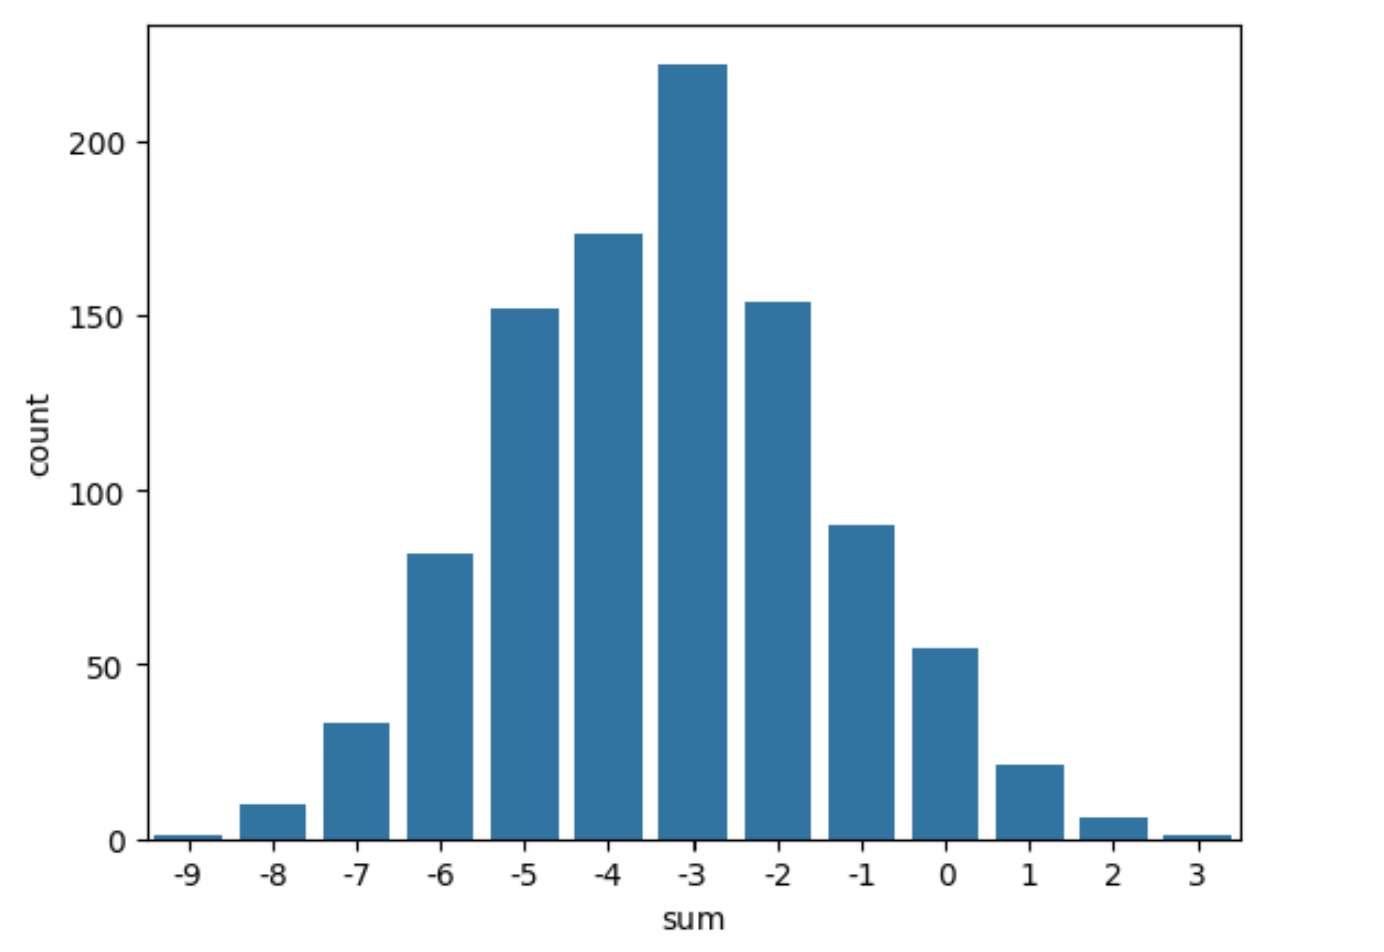
\includegraphics[width=10cm]{figure/figure.png}
    \caption{Distribution for scores of bootstrap resampling.}
    \label{fig:example}
\end{figure}

\\

\begin{table}[ht]
\centering
\begin{tabular}{lll}
\hline
\textbf{Model} & \textbf{Accuracy} & \textbf{F1 score} \\ 
\hline
Baseline Model & 84.6\% & 0.843 \\ 
Experiment Model 2& 51.6\% & 0.540 \\ 
\end{tabular}
\caption{\label{citation-guide}
Accuracy \& F1 Score for each model.
}
\end{table}



\end{document}
